%%%%%%%%%%%%%%%%%%%%%%%%%%%%%%%%%%%%%%%%%%%%
%%% CHYMISTRY
%%%%%%%%%%%%%%%%%%%%%%%%%%%%%%%%%%%%%%%%%%%%



\mysection{Chymistry}{research-chymistry}

The transformation of magic into matter, Chymistry is practiced in Civilization during a Vacation.  Practicing Chymistry requires the Settlement where you're taking the Vacation to have a Library (see the Core Rules).  There are 4 basic kinds of chymicals:

\mylist {
  \item \mybold{Tonics}  are mixtures of booze, narcotics, and other things you probably don't want to know about. They must be drunk
  \item \mybold{Powders} can be drunk (in wine), inhaled, or smoked.  If you blow a powder in some Monster’s face, the Monster has to be able to breathe (so they don't work on undead, for example)
  \item \mybold{Sera} need to be injected via a syringe.  If the recipient is a person, they have to have a vein of some kind.  If the recipient is an object, it has to be something a needle could pierce (like an apple)
  \item \mybold{Unguents} include oils, salves, lubricants, and pastes - basically anything you rub on things (heh heh).  They're usually super viscous and anyone will know the moment they try to drink it.  You can coat a weapon with an unguent  and "apply" it to a Monster by injuring them with the weapon (1 point of damage or more to Flesh).  If your attack misses the unguent doesn't rub off, but if you hit armor / scales / etc. without piercing Flesh, it does.  Unguents can be rubbed on someone who is who is unconscious or petrified.  Can’t be eaten -  tastes shitty and the person will spit it out.
}


  \begin{center}
  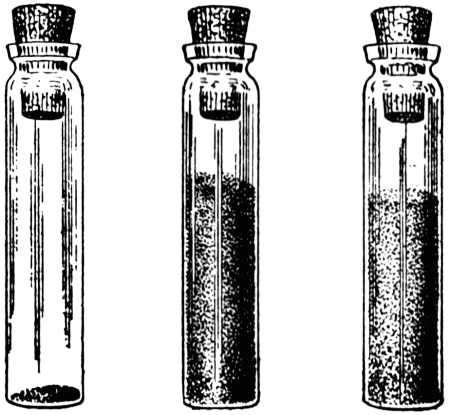
\includegraphics[scale=.5]{Chymistry}
  \end{center}


\mysubsection{Such Mortal Drugs I Have (Toxins)}{research-chymistry-toxins}

You can create a Toxin in the form of a Tonic, Unguent, Sera, or Powder. The efficacy of the potion depends on the type:

  \mytable{X c X} {
    \thead{Craft} & \thead{Damage \& Duration} & \thead{Saves}  \\
  } {
     Iron & d4 & 1  \\
     Silver & d8 & 2  \\
     Gold & d12 & 3  \\
  }

  The die type is the amount of damage over a number of minutes (not Minutes, which is its own unit of time), rolled separately. Thus, a Silver Toxin would deal d8 damage for d8 minutes (the Arbiter is encouraged to roll the duration in secret). Damage hits Grit first (as it wears away your will to live), then Flesh.  You cannot heal Grit while under the effects of a Toxin.  The victim of these Toxins \mybold{always} gets a Save (though see below). 

  When Saving against one of these Toxins, the victim can make a Save every minute \myital{before} they are affected by the damage.  If they make the Save, they do not take damage that minute, BUT the Save does not necessarily end the effect of the Toxin.  In order to shake off the effect of the Toxin, the victim must make a number of rolls equal to the Toxin's Duration.  The Saves do not have to be consecutive. 

  When using a Toxin, you must make a \RS : \DEX or risk poisoning yourself unless you have the Knave Virtue \mybold{Poisonous} (see Core Rules)


  \example {
Andre Preneur (Grit 7, Flesh 6) drinks a Silver Toxin hidden in a glass of wine.  The Arbiter rolls the duration (d8) and gets a 7; the effect will last 7 minutes. The Arbiter starts a timer.  Andre rolls a Save and fails - the Arbiter rolls a d8 and gets a 6.  Andre applies the damage (1 Grit, 6 Flesh).  Another minute passes, Andre rolls a Save and makes it. At the 3rd minute, Andre rolls his Save and fails.  The Arbiter rolls 8 damage.  Andre is now Dying.  He will need to roll his \DEATH every time he takes damage from the Toxin for the next 4 minutes, unless he makes 2 more Saves
  }

  \mysubsection{Potent Waters (Acids)}{research-chymistry-acids}

  In addition to Toxins, you can create various kinds of acids.  Acids are always treated as if they were unguents (though they are on the liquid side), and will dissolve flesh, stone, wood, or metal.  They are often used for etching, ruining locks, and pouring on people you hate.  Like Toxins, you must make a \RS : \DEX when using acids or risk pouring them on yourself.

  \mytable{X c} {
    \thead{Craft} & \thead{\# Effects}  \\
  } {
     Iron & 1  \\
     Silver & 2  \\
     Gold & 3 \\
  }

  Iron acids allow you to pick one of the results below; Silver acids allow you to pick 2; and Gold acids allow you to take all 3.

  \mybullet {
    \item if the acid hits Flesh, deals d4 damage for d4 Moments. If it hits Armor, the Armor \UD must be rolled at the top of every Moment.
    \item the acid can melt an area 100cm cubed of wood, metal, or stone
    \item the acid will create an acrid plume of smoke that causes coughing and choking for Minutes to everything Nearby (-2 to \RO and \RB attempts)
  }

  You can sunder your Shield to negate the effect of acids thrown on you.  

  \cbreak

  \mysubsection{Tonics}{research-chymistry-tonics}

  \CHYMISTRY[
    Name=Chyme's Nerve Tonic,
    Link=chymistry-chymes-nerve-tonic,
    Cost=Iron (1 Research;100\FE),
    Duration=until Bivouac,
    Toxin=No,
    Narcotic=\MAX 1
  ]

  You make all of your \RO and \RB checks at +4, but you can never take a Breather - you're far too restless.  

\CHYMISTRY[
  Name=Cuckhold's Courage,
  Link=chymistry-cuckhold-courage,
  Cost=Iron (1 Research;100\FE),
  Duration=0,
  Toxin=No,
  Narcotic=\MAX 3 
]

Drinking Cuckhold's Courage restores Grit when imbibed during a Breather.  For every bottle of Cuckhold's Courage drunk, the drinker's Grit is healed or increased (even above \MAX !) by +4.  It cannot heal Flesh (only Grit).  Narcotic



\CHYMISTRY[
  Name=Fulcanelli's Clarifying Elixir,
  Link=chymistry-fulcanelli-clarifying-elixir,
  Cost=Silver (3 Research;300\AG),
  Duration=until Bivouac/0,
  Toxin=No,
  Narcotic=No 
]


Renders you almost immune to any spells or effects from the Mind paradigm.  If you wouldn't normally get a Save against the effect, you now do.  If you \mybold{do} get a Save against the effect, the Save is at +4.  If taken while under the effect of a Mind spell, immediately gives the imbiber a Save as above and ends its Duration.  Can be used to break the effects of the Philter of von Fuchs (it is rumored that Fulcanelli was under the sway of von Fuchs)

\CHYMISTRY[
  Name=Liebnitz Purgation,
  Link=chymistry-liebnitz-purgation,
  Cost=Silver (3 Research;300\AG),
  Duration=0 ,
  Toxin=No,
  Narcotic=No 
]

If imbibed while under the effects of an ingested Toxin (Tonic, drunk Powder, or Brew) the poison will be immediately vomited forth intact (d2 \UD) and will cease to affect the victim.  

\CHYMISTRY[
  Name=Philter of von Fuchs,
  Link=chymistry-philter-von-Fuchs,
  Cost=See Below,
  Duration=See Below,
  Toxin=Yes,
  Narcotic=No 
]

When imbibed, the drinker will fall under the sway of whoever gave them the tonic.  Treat as a \mylink{Charm}{wizardry-charm} spell.  Save Negates.  The duration depends on the amount of Research used:  Iron (1), Days; Silver (3), Weeks; Gold (5), Months.  Can be broken by spells, rituals, etc. that relieve effects of the Mind.

  \begin{center}
  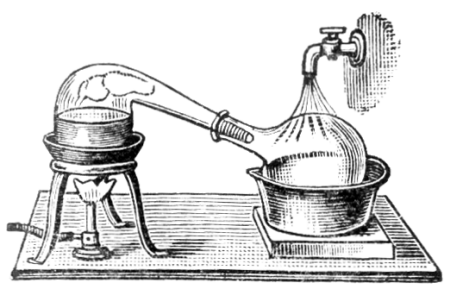
\includegraphics[scale=.5]{Chymistry_2}
  \end{center}


  \mysubsection{Powders}{research-chymistry-powders}

  \CHYMISTRY[
    Name=Dastin's Basic Talc,
    Link=chymistry-dastins-basic-talc,
    Cost=Iron (1 Research;100\FE),
    Duration=0 ,
    Toxin=No,
    Narcotic=No 
  ]


  Sprinkling this powder on something covered in acid immediately neutralizes the acid (damage, etc).


  \CHYMISTRY[
    Name=Mermaid's Kiss,
    Link=chymistry-mermaids-kiss,
    Cost=Silver (3 Research;300\AG),
    Duration=0 ,
    Toxin=Yes,
    Narcotic=No 
  ]


  The imbiber stops breathing for Hours.  They can feign death or travel underwater, are not affected by inhaled powders or gases, and are unable to speak or cast spells.  Unwilling victims get a Save (as if this were a Toxin)



  \CHYMISTRY[
    Name=Powdered Bezoar,
    Link=chymistry-powdered-bezoar,
    Cost=Iron (1 Research;100\FE),
    Duration=0 ,
    Toxin=No,
    Narcotic=No 
  ]


  When sprinkled on a food or into a beverage, has a 5-in-6 chance of neutralizing any Toxin contained inside.  The roll is made in secret by the Arbiter.


  \CHYMISTRY[
    Name=Woundseal,
    Link=chymistry-woundseal,
    Cost=Iron (1 Research;100\FE),
    Duration=0 ,
    Toxin=No,
    Narcotic=No 
  ]


  Sprinkling this powder on a wound stops all effects of Bleeding, like the Leechcraft skill \mylink{Staunch}{leechcraft-staunch}



  \mysubsection{Unguents}{research-chymistry-unguents}
  \CHYMISTRY[
    Name=Boyle's Sharpening Paste,
    Link=chymistry-boyles-sharpening-paste,
    Cost=Iron (1 Research;100\FE),
    Duration=0 ,
    Toxin=No,
    Narcotic=No 
  ]
  When rubbed on the blade of a stabbing or cutting weapon, the weapon deals +d12 the next time damage is rolled.  The oil rubs off after the strike.


  \CHYMISTRY[
    Name=Brahe's Efficacious Sealant,
    Link=chymistry-brahes-efficacious-sealant,
    Cost=Gold (5 Research;500\AU),
    Duration=0 ,
    Toxin=No,
    Narcotic=No 
  ]
  Fast-drying paste. Capable of bonding stone, glass, wood, or metal (but not flesh). Lasts forever.  Can cover an area roughly 10cm square.


  \CHYMISTRY[
    Name=Faivre's Aqua Grease,
    Link=chymistry-faivres-aqua-grease,
    Cost=Iron (1 Research;100\FE),
    Duration=0 ,
    Toxin=No,
    Narcotic=No 
  ]
  A pale grease that can be rubbed over any equipment to completely protect it against damage from water exposure

  \CHYMISTRY[
    Name=Tesla's Silver Wash,
    Link=chymistry-teslas-silver-wash,
    Cost=Silver (3 Research;300\AG),
    Duration=0 ,
    Toxin=No,
    Narcotic=No 
  ]
  When applied to a 1-handed weapon, the weapon becomes permanently imbued with silver.  Requires an ingot of silver.

  \CHYMISTRY[
    Name=Wei Boyang's Alkahest,
    Link=chymistry-wei-boyangs-alkahest,
    Cost=Gold (5 Research;500\AU),
    Duration=0 ,
    Toxin=No,
    Narcotic=No 
  ]

  This oil will dissolve any adhesive (including Brahe's Efficacious Sealant).  Can cover an area roughly 10cm square.


\mysubsection{Sera}{research-chymistry-sera}

  \CHYMISTRY[
    Name=Al-Farabi's Calming Injection,
    Link=chymistry-al-farabis-calming-injection,
    Cost=Gold (5 Research;500\AU),
    Duration=0 ,
    Toxin=Yes,
    Narcotic=No 
  ]

  The injected creature ceases immediately to be Enraged, Shaken, Frenzied, or Disgusted.  If the creature is Zoological, they become passive and docile.  Creatures under the effect of the Calming Injection cannot attack unless they are attacked first.  Lasts for Hours. Unwilling creatures get a Save to negate.

  \CHYMISTRY[
    Name=Davy's Soothing Anesthetic,
    Link=chymistry-davys-soothing-anesthetic,
    Cost=Silver (3 Research;300\AG),
    Duration=0 ,
    Toxin=Yes,
    Narcotic=No 
  ]

  The injected creature feels any pain as pleasure for Hours.  Often surreptitiously given to those undergoing torture, or going under the knife for surgery.  Attacks against the recipient ignore Grit as the mind loses the cues to shift away from painful events.  


  \CHYMISTRY[
    Name=Grimm's Stupurous Preparation,
    Link=chymistry-grimms-stupurous-preparation,
    Cost=Gold (5 Research;500\AU),
    Duration=0 ,
    Toxin=Yes,
    Narcotic=No 
  ]


  An injected creature immediately falls into a slumber in all ways like \mylink{Sleep}{wizardry-sleep} (can't be awakened except by a slap, doesn't effect a creature of greater than 4 \HD) unless they Save

  If the sera is injected into solid food of some sort (like an apple), any creature ingesting the food falls into a deep slumber and cannot be awakened except by a Mystic feeding the curse to a 3+ Cunning \mylink{Hekaphage}{occultism-hekaphage}. While asleep the creature is in a state of suspended animation - they do not age, and do not need to eat or drink - but they can still be killed in the normal means (dagger through the heart, etc).  Putting a creature into suspended animation will stop the effects of progressing disease and toxins.  Unwilling creatures get a Save. 

  \CHYMISTRY[
    Name=Wordwarp,
    Link=chymistry-wordwarp,
    Cost=Gold (5 Research;500\AU),
    Duration=0 ,
    Toxin=Yes,
    Narcotic=No 
  ]

  An oil that causes a form of dyslexia.  If the victim fails a Save, they are unable to read written words for Hours.  Often used on spell casters and scribes.


\newpage

